\documentclass[12pt]{book}
\usepackage[a4paper,bindingoffset=0.2in,%
            left=0.75in,right=0.75in,top=1in,bottom=1in,%
            footskip=.25in]{geometry}
\usepackage{fancyhdr}
\setlength{\headheight}{15.2pt}
\usepackage[utf8]{inputenc}
\pagestyle{fancy}

\renewcommand{\chaptermark}[1]{\markboth{\thechapter.\ #1}{}}
\renewcommand{\sectionmark}[1]{\markright{\thesection\ #1}}
\fancyhead[LE,RO]{\textbf{\thepage}}
\fancyhead[LO]{\textbf{\rightmark}}
\fancyhead[RE]{\textbf{\leftmark}}
\fancyfoot{}
\fancypagestyle{plain}
{
    \fancyhf{}
}


\usepackage{amsmath}
\usepackage{amssymb}
\usepackage{mathtools}
\usepackage{xcolor}
\usepackage{enumitem}
\usepackage{graphicx}
\usepackage[noend , noline, ruled]{algorithm2e}
\usepackage{pgfplots}
\pgfplotsset{width=7cm,compat=1.18}

\usepgfplotslibrary{external}
\tikzexternalize%[prefix=TikzPDFs/]

\usepackage{common}
\usepackage{english-theorems}
\setcounter{tocdepth}{1}
        
\begin{document}
\tableofcontents
\clearpage
\ifodd\value{page}\else
\thispagestyle{empty}
\fi
\chapter{Introduction}
Cryptography is the art and science of encrypting and decrypting a message. 
\section{Symmetric cipher}
A symmetric cipher scheme \(\Pi\) can be viewed as a triplet \(\bracket{\Gen, \Enc , \Dec}\) of algorithms. Suppose \(\Messages\) be the set of all possible messages and \(\Keys\) be the set of all keys. \(\Gen\) chooses a key \(k \in \Keys\) and then \(\Enc : \Messages \times \Keys \to \Ciphers\) encrypts the message \(m\) with key \(k\) and returns the cipher \(c\). Lastly, \(\Dec: \Ciphers \times \Keys \to \Messages \cup \but\) decrypts the cipher \(c\) with key \(k\) and returns either a message or an error, denoted as \(\but\). Without loss of generality we can assume that \(\Gen\) picks \(k\) uniformly from \(\Keys\). Futhermore, \(\Enc\) can be randomized, however \(\Dec\) is deterministic and for every message \(m\) and key \(k\) we must have 
\begin{equation*}
    \func{\Dec_k}{\func{\Enc_k}{m}} = m
\end{equation*}

\section{Kerckhoff's principle}
Kerckhoff's principle assumes the following for every encryption scheme 
\begin{enumerate}
    \item The encryption and decryption is known to everyone.
    \item The security of the scheme is only dependent on the key.
\end{enumerate}

\section{Prefectly secret encryption}
Let \(K\) and \(M\) be two random variables, where \(K\) is the result of \(\Gen\) and \(M\) is the message. We can assume that they are independent. Furthermore, \( C = \func{\Enc_K}{M}\) is also a random varible. By the Kerckhoff's principle, we assume that the distribution on \(M\) and \(\Enc\) is known and only \(K\) is unknown. 

\begin{definition}[Perfectly secure encrption]
    An encryption scheme is perfectly secure if for all \(c \in \Ciphers\) with \(\prob{C = c} > 0\):
    \begin{equation}
        \forall m \in \Messages, \quad \condProb{M = m}{C = c} = \prob{M = m}
    \end{equation}
 \end{definition} 

 \begin{proposition}
     An encryption scheme \(\Pi\) is perfectly secure if and only if 
     \begin{equation}
         \forall m,m' \in \Messages, \quad \prob{\func{\Enc_K}{m} = c} = \prob{\func{\Enc_K}{m'} = c}
     \end{equation}
 \end{proposition}

 \begin{proof}
     Suppose \(\Pi\) is perfectly secure then (assuming that \(\prob{M = m} > 0\))
     \begin{align*}
         \prob{\func{\Enc_K}{m} = c} &=  \condProb{C = c}{M = m} = \dfrac{\condProb{M = m}{C = c} \prob{C = c}}{\prob{M = m}}\\
         &= \dfrac{\prob{M = m} \prob{C= c}}{\prob{M= m}} = \prob{C = c}
     \end{align*}
     Now if the equation holds for \(\Pi\) then (again assuming that \(\prob{M = m} > 0 \))
     \begin{align*}
        \condProb{M = m}{C = c} &= \dfrac{\condProb{C = c}{M = m} \prob{M = m}}{\prob{C = c}}\\
        &= \dfrac{\func{\Enc_K}{m} \prob{M = m}}{\sum_{m^{\ast}} \condProb{C = c}{M = m^{\ast}} \prob{M = m^{\ast}}}\\
        &= \dfrac{\prob{M = m}}{\sum_{m^{\ast}} \prob{M = m^{\ast}}} = \prob{M = m}
     \end{align*}
 \end{proof}
%\chapter{Classifier}
To predict, we come up with a \textbf{hypothesis}. A hypothesis is a parametrized function that maps input to output
\begin{equation*}
    y = \func{h}{x ; \theta} , \qquad h \in \CalH, \theta \in \Theta
\end{equation*}
where \(\CalH\) is our \textit{hypothesis class}. We wish to find the parameters \(\theta\) that matches our data well. One way to evaluate how well our hypothesis predicts is to introduce a \textbf{loss function} (or \textit{cost function}), \(\func{L}{a,a_h}\) where \(a,a_h\) are in the output set and the loss function assigns a value to how close our prediction \(a_h\) when the actual value is \(a\). We wish that our hypothesis to have the least loss on new data.
\begin{equation*}
    \func{\CalE}{h} = \dfrac{1}{n'} \sum_{i = n + 1}^{n + n'} \func{L}{\func{h}{x^{(i)} ; \theta }, y^{(i)}}
\end{equation*}
One way to do this is minimize the training error 
\begin{equation*}
    \func{\hat{\CalE}}{h} = \dfrac{1}{n} \sum_{i = 1}^n \func{L}{\func{h}{x^{(i)} ; \theta }, y^{(i)}}
\end{equation*}
There are several types of loss function
\begin{description}
    \item[0-1 Loss]
        \begin{equation*}
            \func{L}{a,a_h} = \begin{cases}
                0 & \text{if} \quad a = a_h \\
                1 & \text{otherwise}
            \end{cases}
        \end{equation*}
    \item[Squared loss]
        \begin{equation*}
            \func{L}{a,a_h} = (a - a_h)^2
        \end{equation*}
    \item[Linear loss]
        \begin{equation*}
            \func{L}{a,a_h} = \abs[a - a_h]
        \end{equation*}
    \item[Asymmetric loss] For example, maybe guessing negative wrong is costlier than guessing positive wrongly, in a binary classification problem.
\end{description}
The model we use, typically, selects \(h\) and we need to minimize the loss (or any other optimization) on the \(\theta\) so that our prediction \textit{fits} the data. To determine a good \(\theta\) we need algorithms, \textit{learning algorithms}. Given a classifier \(h\) we can easily evaluate its performance by testing it on new data. However, to evaluate a learning algorithm we have to first train it on some data and then evaluate the resulting classifier on the testing data. Doing this multiple gives us an estimate of how well the algorithm works. In most cases, we do not have access to a lot of data (we don't now the distribution). In these cases we can re-use data using cross validation 


\begin{algorithm}[H]
    \DontPrintSemicolon
    divide $\CalD$ into $k$ equally sized chunks  $\CalD_1 , \dots , \CalD_k$ \;
    \For{$i= 1 \to k$}{
        train $h_i$ on $\CalD - \CalD_i$\;
        compute $\func{\CalE_i}{h_i}$ on the test data $\CalD_i$\;
    }
    \Return{$\frac{1}{k} \sum_{i = 1}^k \func{\CalE_i}{h_i}$}
    \caption{ cross\_validate $(\CalD , k )$}
\end{algorithm}

\section{Linear classifiers}
A linear classifier has the following form
\begin{equation*}
    \func{h}{x; \theta , \theta_0} = \func{\sign}{\theta^T x + \theta_0} \qquad \theta \in \Reals^d , \theta_0 \in \Reals
\end{equation*}

\subsection{Random linear classifier}
One way to select the parameters \(\theta\) and \(\theta_0\) is to randomly select them and return the best one.

\begin{algorithm}[H]
    \DontPrintSemicolon
    \For{$j= 1 \to k$}{
        $\theta^{(j)} = $Random$(\Reals^d)$ \;
        $\theta^{(j)}_0 = $Random$(\Reals)$ \;
    }
    $j^\ast = \argmin_{\substack{1 \leq j \leq k}} \func{\hat{\CalE}}{\func{h}{x, \theta^{(j)} , \theta^{(j)}_0}}$

    \Return{$(\theta^{(j^\ast)} , \theta^{(j^\ast)}_0)$}
    \caption{ random\_linear\_classifier $(\CalD_n , k )$}
\end{algorithm}

\subsection{Perceptron}
A more intelligent way of finding the parameters is to update when we encounter a mistake. The simplest update rule is the \textbf{perceptron} \footnote{the perceptron algorithm introduced here is the stochastic version, the batch version can be easily arrived.}, which is as follows
\begin{equation*}
    \theta' ,\; \theta_0' \gets \theta + y^{(i)}x^{(i)} ,\; \theta_0 + y^{(i)}
\end{equation*}
This update increase the magnitude of \(y^{(i)}\cdot(\theta^T x^{(i)} + \theta_0)\) as shown below, and hence in enough iterations, the sign will become positive.

\begin{align*}
    y^{(i)}\cdot  \left( \theta^{'T} x^{(i)} + \theta'_0 \right) &= y^{(i)} \left( \theta + y^{(i)} x^{(i)} \right)^T x^{(i)} + y^{(i)} \left( \theta_0 + y^{(i)} \right)\\
    &= y^{(i)} \cdot \left( \theta^T x^{(i)} + \theta_0 \right) + (y^{(i)})^2 \left( \norm[x^{(i)}]^2 + 1 \right)\\
    &=  y^{(i)} \cdot\left( \theta^T x^{(i)} + \theta_0 \right)+ \norm[x^{(i)}]^2 + 1
\end{align*}
however it is not clear how other mistakes will affect the current guess.

\begin{algorithm}[H] \label{algo:perceptron}
    \DontPrintSemicolon
    $\theta = 0 $\;
    $\theta_0 = 0 $\;
    \For{$t= 1 \to T$}{
        \For{$i = 1 \to n$}{
            \If{ $y^{(i)} (\theta^T x^{(i)}) + \theta_0 \leq 0$}{
                $\theta = \theta +  y^{(i)} x^{(i)}$ \;
                $\theta_0 = \theta_0 + y^{(i)} $\;
            }
        }
    }

    \Return{$(\theta , \theta_0)$}
    \caption{ perceptron $(\CalD_n , T )$}
\end{algorithm}


By adding another dimension to our data set we can simplify our prediction to pass through the origin
\begin{align*}
    x'       & = \begin{bmatrix}
        x_1 & \dots & x_n & 1
    \end{bmatrix}, \qquad \theta' = \begin{bmatrix}
        \theta & \theta_0
    \end{bmatrix} \\
    \implies & \theta^{'T} x' = \theta^T x + \theta_0
\end{align*}

Therefore, one can also simplify the \Cref{algo:perceptron} to the following

\begin{algorithm}[H]
    \DontPrintSemicolon
    $\theta = 0 $\;
    \For{$t= 1 \to T$}{
        \For{$i = 1 \to n$}{
            \If{ $y^{(i)} (\theta^T x^{(i)}) + \theta_0 \leq 0$}{
                $\theta = \theta +  y^{(i)} x^{(i)}$ \;
            }
        }
    }

    \Return{$\theta $}
    \caption{ perceptron $(\CalD_n , T )$}
\end{algorithm}

To examine the convergence of the perceptron algorithm we need the following definitions. A dataset \(\CalD_n\) is \textbf{linearly separable -through the origin} if there is some \(\theta\) such that
\begin{equation*}
    y^{(i)} \theta^T x^{(i)} > 0 \quad \forall i
\end{equation*}
and similary it is linearly separable if there are some \(\theta , \theta_0\) such that 
\begin{equation*}
    y^{(i)} \cdot \left( \theta^T x^{(i)}  + \theta_0 \right) > 0 \quad \forall i
\end{equation*}
The \textbf{margin} of a labeled data point \((x,y)\) with respect to a separator (hyperplane) \(\theta, \theta_0\) is
\begin{equation*}
    y \cdot \dfrac{\theta^T x +  \theta_0}{\norm[\theta]}
\end{equation*}
which basically quantifies how we \(\theta\) approximates the data point \((x,y)\) in a data set \(\CalD_n\). Also the margin of \(\CalD_n\) w.r.t \(\theta, \theta_0\) is
the minimum of all margins:
\begin{equation*}
    \min_i     y^{(i)} \cdot \dfrac{\theta^T x^{(i)} + \theta_0}{\norm[\theta]}
\end{equation*}

\begin{theorem} [Perceptron convergence theorem] \footnote{also applys to batch version}
    If there exists a vector \(\theta^\ast\) such that the margin of database with respect to \(\theta^\ast\) is greater than \(\gamma > 0\) and then norm \(\norm[x^{(i)}] \leq R\) for some \(R\) then perceptron will make at most \(\left(\frac{R}{\gamma} \right)^2\) updates/mistakes.
\end{theorem}

\begin{proof}
    The idea of the proof is to put an increasing lower bound on the cosine of the angle between the \(k_{\cardinalTH}\) update \(\theta^{(k)}\) and \(\theta^{\ast}\). Note that 
    \begin{equation*}
        \func{\cos}{\angle \theta^{\ast} , \theta^{(k)}} = \dfrac{(\theta^{\ast})^T \theta^{(k)}}{\norm[\theta^{\ast}] \norm[\theta^{(k)}]}
    \end{equation*}
    we know that for some \(i\), \(\theta^{(k)} = \theta^{(k - 1)} + y^{(i)} x^{(i)}\), then 
    \begin{align*}
        (\theta^{\ast})^T \theta^{(k)} &= (\theta^{\ast})^T \left(\theta^{(k- 1)} + y^{(i)} x^{(i)} \right) \\
        &=(\theta^{\ast})^T \theta^{(k- 1)}+   y^{(i)} (\theta^{\ast})^T x^{(i)} \\
        &\geq  (\theta^{\ast})^T \theta^{(k- 1)} + \gamma \norm[\theta^{\ast}]\\
        &\geq  k \gamma \norm[\theta^{\ast}]
    \end{align*}
    also 
    \begin{align*}
        \norm[\theta^{(k)}]^2 &=  \left(\theta^{(k- 1)} + y^{(i)} x^{(i)} \right)^T  \left(\theta^{(k- 1)} + y^{(i)} x^{(i)} \right)\\
        &= \norm[\theta^{(k-1)}]^2 + 2y^{(i)} (\theta^{(k-1)})^T x^{(i)} + \left( y^{(i)}\right)^2 \norm[x^{(i)}]^2 \\
        &\leq  \norm[\theta^{(k-1)}]^2 +  \norm[x^{(i)}]^2 \\
        &\leq  \norm[\theta^{(k-1)}]^2 + R^2 \\
        &= kR^2
    \end{align*}
    therefore 

    \begin{equation*}
        \func{\cos}{\angle \theta^{\ast} , \theta^{(k)}} \geq \sqrt{k} \; \frac{\gamma}{R}
    \end{equation*}
    Since the cosine can not exceed one therefore the we at most make 

    \begin{equation*}
        k \leq \left(\dfrac{R}{\gamma}\right)^2 
    \end{equation*}
    mistakes.
    For a linearly inseparable we can remember the best \(\Theta\) and after some iteration return that.
 \end{proof}

 \section{Linear Discriminant Analysis}
 In Fisher's LDA we are looking for a vector that when the samples are projected on that vector, they are well separated. One objective could be maximizing the distance of average positions of the classes from each other. Assuming the norm of the vector  \(\norm[\theta] = 1\) then our the average position of projected samples for each class is 
 \begin{align*}
     \mu_1 &= \dfrac{\sum_{x^{(i)} \in \CalC_1} x^{(i)}}{\abs[\CalC_1]}\\
     \mu_2 &=\dfrac{\sum_{x^{(i)} \in \CalC_2} x^{(i)}}{\abs[\CalC_2]}\\
     \psi_1 &=  \theta^T \mu_1 , \quad \psi_2 = \theta^T \mu_2
 \end{align*}
 Then mathematically our objective is 
 \begin{equation*}
     \max_{\theta} \func{J}{\theta} = \max_{\theta} (\psi_1 - \psi_2)^2
 \end{equation*}
 Solving this analytically using the Lagrange multiplies gives 

\begin{equation*}
    \nabla_{\theta} \func{J}{\theta} + \lambda (\norm[\theta] - 1) = 2 (\psi_1 - \psi_2)(\mu_1 - \mu_2) - \lambda \theta = 0
\end{equation*}
Therefore \(\theta\) is in the same direction as \(\mu_1 - \mu_2\) hence it must be  
\begin{align*}
    \theta &= \dfrac{\mu_1 - \mu_2}{\mu_1 - \mu_2}
\end{align*}

The problem with this approach is that it doesn't consider the variance of the samples. Hence, it is possible that even though our separator maximizes the distance between the two averages, it still misclassifies a lot of points. In order to take variance into account we change our objective to the following

\begin{equation*}
    \func{J}{\theta} = \dfrac{(\psi_1 - \psi_2)^2}{\sigma_1^2 + \sigma_2^2}
\end{equation*}
where 
\begin{align*}
    \sigma_1^2 &= \sum_{x^{(i)} \in \CalC_1} \left(\theta^T x^{(i)} - \theta^T \mu_1 \right)\\
    \sigma_2^2 &= \sum_{x^{(i)} \in \CalC_2} \left(\theta^T x^{(i)} - \theta^T \mu_2 \right)
\end{align*}

We can simplify our objective to have the following form
\begin{equation*}
    \func{J}{\theta} = \dfrac{\theta^T S_B \theta}{\theta^T S_W \theta }
\end{equation*}
where 
\begin{align*}
    S_B &= (\mu_1 - \mu_2) (\mu_1 - \mu_2)^T\\
    S_W &= \sum_{x^{(i)} \in \CalC_1} (x^{(i)} - \mu_1)(x^{(i)} - \mu_1)^T + \sum_{x^{(i)} \in \CalC_2} (x^{(i)} - \mu_2)(x^{(i)} - \mu_2)
\end{align*}
Which are between-class scatter matrix and within-class scatter matrix respectively. Taking the derivative with respect to \(\theta\) and setting it to zero 
\begin{equation*}
    S_B \theta = \lambda S_w w
\end{equation*}
for some constant \(\lambda\). Note that 
\begin{equation*}
    S_B \theta = (\mu_1 - \mu_2) (\mu_1 - \mu_2)^T \theta = a (\mu_1 - \mu_2)
\end{equation*}
hence 
\begin{equation*}
    w = b S_W^{-1} (\mu_1 - \mu_2)
\end{equation*}

\section{Features}
\subsection{Transformation}
As we saw we can transform linearly separable dataset to another linearly separable dataset but without an offset. What happens if the original dataset is not linearly separable? For example, \textit{xor dataset}:
\begin{figure*}[!ht]
    \centering
    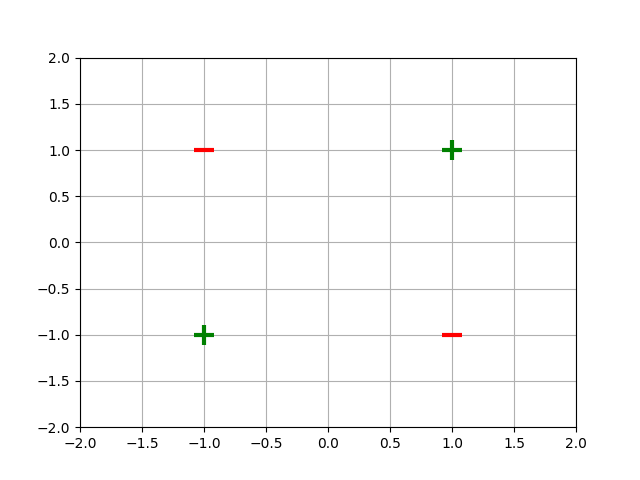
\includegraphics{Chapters/graphics/xor_dataset.png}
    \caption{XOR dataset}
\end{figure*}

\begin{equation*}
    \CalD = \set{((-1,-1),1), ((-1,1), -1) , ((1,-1),-1) , ((1,1),1)}
\end{equation*}
is not linearly separable in 2 dimensions. A transformation that might be applicable here is \textbf{polynomial basis}. A polynomial basis transformation of order \(k\), transforms a feature \(x \in \Reals^d\) to
\begin{equation*}
    \func{\phi}{x} = ( x_1^{\alpha_1} \dots x_d^{\alpha_d}) , \quad \sum_{i = 1}^d \alpha_i \leq k , \forall i, \alpha_i \geq 0
\end{equation*}
which has \(\binom{k + d }{d }\) dimension.

For example, the transformation \(\func{\phi}{x_1, x_2} = (x_1,x_2,x_1x_2)\) makes the xor dateset linearly separable-through the origin.
\begin{figure*}[!ht]
    \centering
    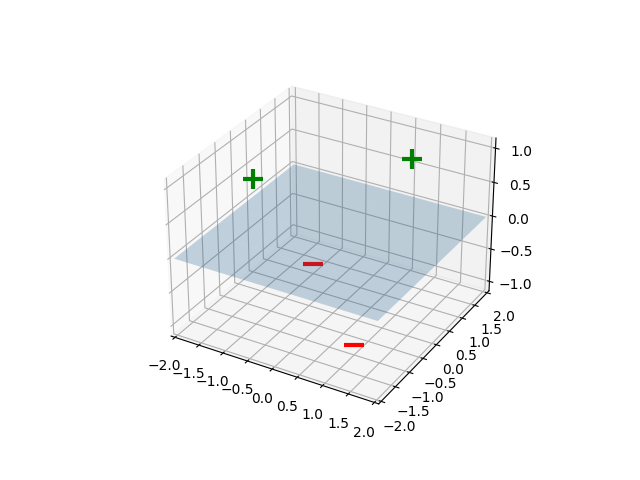
\includegraphics{Chapters/graphics/xor_3d.png}
    \caption{Transformed XOR dataset}
\end{figure*}
\subsection{Representation}
we can represent a discrete feature as
\begin{enumerate}
    \item numeric
    \item thermometer code (a vector of \(m\) booleans where \(1\dots j\) bits are on and the rest or off)
    \item one-hot (a vector of \(m\) booleans where \(j_{\cardinalTH}\) bit is on adn the rest are off)
    \item factoring (group information of a feature based its structure maybe)
\end{enumerate}

For numeric feature we would like to standardized as follow
\begin{equation*}
    \tilde{x_j}  = \dfrac{x_j - \bar{x_j}}{\sigma}
\end{equation*}

\section{Multi-class classification}
One way is to reduce the problem to multiple binary classification problem. However, this method can lead to regions in which classification is ambiguous.
Another way to solve the multi-class classification is to design a function \(f_i\) for each class \(\CalC_i\) then classifiying new data could be done using 
\begin{equation*}
    y = \argmax_i \func{f_i}{x}
\end{equation*}
%\chapter{Logistic Regression}
In machine learning we wish to optimize a function like \(\func{J}{\theta}\). Usually a function in form
\begin{align*}
    \func{J}{\theta} & = \left(\dfrac{1}{n} \sum_{i = 1}^n \func{L}{\func{h}{x^{(i)}; \theta} , y^{(i)}} \right) + \lambda \func{R}{\theta} \\
                     & = \CalE_n + \lambda \func{R}{\theta}
\end{align*}
where \(R\) is the \textbf{regularization function} and \(\lambda\) is a hyperparameter. A common regularizer is
\begin{equation*}
    \func{R}{\theta} = \norm[\theta - \theta_{\mathrm{prior}}]^2
\end{equation*}
where \(\theta_{\mathrm{prior}}\) is the value that we want \(\theta\) to be close to.

\section{Linear logistic classifier}
The problem of minimizing 0-1 Loss problem is NP-hard. A problem with sign is that incremental change are hard to find because of the discrete nature of the function hence, to smooth out the sign function we use \text{sigmoid} function
\begin{equation*}
    \func{\sigma}{x} = \dfrac{1}{1 + e^{-x}}
\end{equation*}
\tikzsetnextfilename{Chapters/graphics/sigmoid/sigmoid_function}
\begin{center}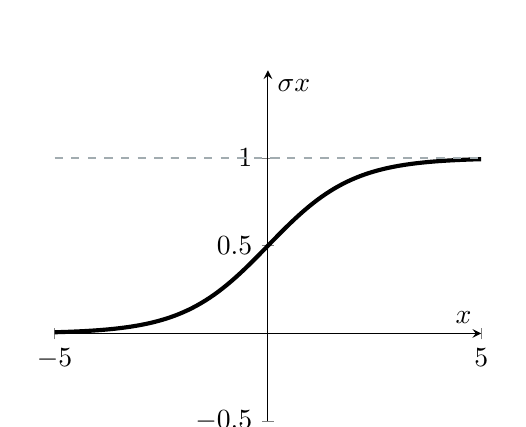
\begin{tikzpicture}
        \begin{axis}[
                axis lines = center,
                xlabel = \(x\),
                ylabel = {\(\func{\sigma}{x}\)},
                xmin = -5, xmax = 5,
                ymin = -0.5 , ymax = 1.5,
                xtick ={-5,0,5},
                ytick = {-0.5,0,0.5,1}
            ]
            \addplot [
                line width = 1.5,
                domain=-5:5,
                samples=100,
                color=black,
            ]
            {1/(1 + e^(-x))};
            \definecolor{grey}{rgb}{0.635, 0.674, 0.690}   
            \addplot [
                line width = 0.8,
                domain= -5:5,
                samples = 100,
                color = grey,
                dashed, 
                ]{1.0};
        \end{axis}
\end{tikzpicture}
\end{center}


Equivalently, we want to make classifier that predict \(+1\) when \(\func{\sigma}{\theta^T x+ \theta_0} > p = 0.5\) and \(-1\) otherwise. The value \(p\) is called the \textbf{prediction threshold}.

Loss on all data is inversely related to the probability that \((\theta , \theta_0)\) assigns to the data. Assuming that points in data set are independent.

\begin{align*}
    g^{(i)} & =  \func{\sigma}{\theta^T x + \theta_0} \\
    p^{(i)} & = \begin{cases}
        g^{(i)}     & \text{if} \quad y^{(i)} = 1 \\
        1 - g^{(i)} & \text{if} \quad y^{(i)} = 0 \\
    \end{cases}
\end{align*}
and we wish to maximize the probability (\(\Theta\) here means \((\theta, \theta_0)\)):
\begin{equation*}
    \func{p}{\Theta ; \CalD_n} = \prod_{i = 1}^n p^{(i)} = \prod_{i = 1}^n (g^{(i)})^{y^{(i)}} ( 1 - g^{(i)})^{(1 - y^{(i)})}                   \\
\end{equation*}

Using the log-likelihood
\begin{equation*}
    \implies \func{\CalL_{LL}}{p} = \sum_{i = 1}^n \func{\CalL_{LL}}{g^{(i)} , y^{(i)}} =\sum_{i = 1}^n  y^{(i)} \func{\ln}{g^{(i)}} + \left(1 - y^{(i)} \right) \func{\ln}{ 1 - g^{(i)}} 
\end{equation*}
then our loss function would be
\begin{equation*}
    \func{L}{\func{h}{x^{(i)}, \Theta} , y^{(i)}} = - \func{\CalL_{LL}}{g^{(i)} , y^{(i)}} =\func{\CalL_{NLL}}{g^{(i)} , y^{(i)}} 
\end{equation*}

hence we wish to minimize the 

\begin{equation*}
    \func{J}{\Theta}  = \left(\dfrac{1}{n} \sum_{i = 1}^n \func{\CalL_{NLL}}{ \func{\sigma}{\theta^T x^{(i)} + \theta_0} , y^{(i)}} \right) + \lambda \norm[\theta]^2
\end{equation*}

note that we didn't include \(\theta_0\) in the regularizer as we don't want to punish large \(\theta_0\). 

\section{Gradient descent}
\subsection{Batch gradient descent}
\begin{algorithm}[H]
    \DontPrintSemicolon
    $\theta^{(0)} = \theta_{\mathrm{init}} $\;
    $t = 0 $\;

    \Repeat{$\abs[\func{f}{\theta^{(t)}} - \func{f}{\theta^{(t - 1)}}] < \epsilon $}{
        $ \theta^{(t)} = \theta^{(t-1)} - \eta \func{\nabla f}{\theta^{(t-1)}} $\;
    }

    \Return{$\theta $}
    \caption{batch gradient descent $(f, \nabla f, \theta_{\mathrm{init}} , \eta , \epsilon )$}
\end{algorithm}

\begin{theorem}
    If \(f\) is convex, for any desired accuracy \(\epsilon\) there is some \(\eta\) such that batch gradient descent will converge to \(\theta\) within \(\epsilon\) of the optimum.
\end{theorem}

Lets derive the closed form of gradient descent for the logistic regression \(J\) function. 
\begin{equation*}
    \nabla \func{J}{\Theta} = \left(\dfrac{1}{n} \sum_{i = 1}^n \nabla \func{\CalL_{NLL}}{ \func{\sigma}{\theta^T x^{(i)} + \theta_0} , y^{(i)}} \right) + \lambda \nabla \norm[\theta]^2
\end{equation*}
we have that 
\begin{align*}
    \PDiff{\func{\CalL_{NLL}}{g^{(i)} , y^{(i)}}}{\theta_j} &= - \dfrac{y^{(i)}}{g^{(i)}} \PDiff{g^{i}}{\theta_j} + \dfrac{1- y^{(i)}}{1 - g^{(i)}} \PDiff{g^{i}}{\theta_j}\\
    &= \dfrac{g^{(i)} - y^{(i)}}{g^{i} \left( 1 - g^{(i)} \right)} \ODiff{\sigma(z)}{z} \PDiff{z}{\theta_j} \\
    \intertext{for simplicity assume \(x^{(i)}_0 = 1\)}
    &= \dfrac{g^{(i)} - y^{(i)}}{g^{i} \left( 1 - g^{(i)} \right)} \left(g^{(i)} - \left(g^{(i)}\right)^2 \right) x^{(i)}_j\\
    &= \left(g^{(i)} - y^{(i)}\right) x^{(i)}_j \\
    \implies \nabla \func{\CalL_{NLL}}{g^{(i)} , y^{(i)}} &=\left(g^{(i)} - y^{(i)}\right) x^{(i)} \\
    \intertext{also for the regularizer}
    \PDiff{\norm[\theta]^2}{\theta_j} &= \begin{cases}
        2 \theta_j & j \neq 0\\
        0 & j = 0
    \end{cases}
\end{align*}

Therefore, 

\begin{align*}
    \nabla_{\theta} \func{J}{\Theta} &= \left(\dfrac{1}{n} \sum_{i = 1}^n \left(g^{(i)} - y^{(i)}\right) x^{(i)} \right) + 2\lambda \theta\\
    \nabla_{\theta_0} \func{J}{\Theta} &= \dfrac{1}{n} \sum_{i = 1}^n g^{(i)} - y^{(i)} 
\end{align*}

\subsection{Stochastic gradient descent}
Suppose we want to minimize \(\func{f}{\Theta}\) which can be written as a sum of some \(\func{f_i}{\Theta}\)
\begin{equation*}
    \func{f}{\Theta} = \sum_{i = 1}^n \func{f_i}{\Theta}
\end{equation*}
Instead of adding up the gradient for each part every iteration, we can choose one of the functions and apply the gradient descent for that function only. We expect that running this algorithm for long enough gives us the optimum solution just like the gradient descent.

\begin{algorithm}[H]
    \DontPrintSemicolon
    $\Theta^{(0)} = \Theta_{\mathrm{init}} $\;
    \For{$t = 1 \to T $}{
        $i = $Random$(\set{1, \dots , n})$\; 
        $ \Theta^{(t)} = \Theta^{(t-1)} - \func{\eta}{t} \func{\nabla f_i}{\theta^{(t-1)}} $\;
    }

    \Return{$\theta $}
    \caption{stochastic gradient descent $(f, \nabla f_1 , \dots,  \nabla f_n, \Theta_{\mathrm{init}} , \eta , T )$}
\end{algorithm}

\begin{theorem}
    If \(f\) is convex and \(\func{\eta}{t}\) is sequence satisfying 
    \begin{equation*}
        \sum_{i= 1}^n \func{\eta}{t} = \infty \quad \mathrm{and} \quad \sum_{i= 1}^n \func{\eta^2}{t} < \infty
    \end{equation*}
    Then SGD converges almost sure to the optimal \(\Theta\).
\end{theorem}

\section{Linear regression}
In regression our output is a real number as oppose to a discrete value. Typically, we use \textit{squared error} for loss function.
\begin{equation*}
    \func{L}{g^{(i)}, y^{(i)}} = \left(g^{(i)} - y^{(i)}\right)^2
\end{equation*}

and hence our \(J\) function will be the \textit{mean squared error} 

\begin{equation*}
    \func{J}{\Theta} = \dfrac{1}{n} \sum_{i = 1}^n \left( g^{(i)} - y^{(i)} \right)^2 + \lambda \func{R}{\Theta}
\end{equation*}

\subsection{Linear hypothesis}
Discarding \(\theta_0\) (for simplicity) and the regularizer term and by allowing our hypothesis \(h\) to be linear --- that is \(g^{(i)} = \func{h}{x^{(i)}; \theta} = \theta^T x\)---, we can easily arrive at a closed form optimal solution. To do this consider the following definitions 
\begin{equation*}
    X = \begin{bmatrix}
        x^{(1)}_1 & \dots & x^{(1)}_d \\
        \vdots & \ddots & \vdots\\
        x^{(n)}_1 & \dots & x^{(n)}_d
    \end{bmatrix} \qquad Y = \begin{bmatrix}
        y^{(1)}\\
        \vdots \\
        y^{(n)} 
    \end{bmatrix}
\end{equation*}

then we can write \(\func{J}{\theta}\) as

\begin{equation*}
    \func{J}{\theta} = \frac{1}{n} (X\theta - Y)^T (X\theta-Y)
\end{equation*}
taking the gradient gives 
\begin{align*}
    \nabla \func{J}{\hat{\theta}} &= \dfrac{2}{n} X^T (X\hat{\theta} - Y) = 0\\
    \implies  X^T X\hat{\theta} &= X^T Y \implies \hat{\theta} = \left(X^T X\right)^{-1} X^T Y
\end{align*}
Assuming the invertibility of \(X^TX\), this minimizes the \(J\) function. However, we will run into the problem of \textit{overfitting}. By adding the regularizer back we can solve the problem of invertibility and overfitting at the same time. Consider the following \(J_{\mathrm{ridge}}\) function, 
\begin{align*}
    \func{J_{\mathrm{ridge}}}{\theta} &= \frac{1}{n} (X\theta - Y)^T (X\theta-Y) + \lambda \theta^T \theta \\
     \implies \nabla \func{J_{\mathrm{ridge}}}{\hat{\theta}} &= \dfrac{2}{n} X^T (X\hat{\theta} - Y) + 2\lambda \hat{\theta}  = 0\\ 
     \implies  (X^TX + n \lambda I) \hat{\theta} &= X^T Y \implies \hat{\theta}  = (X^TX + n \lambda I )^{-1} X^T Y
\end{align*}

A faster way of computing the optimal solution is using the SGD or BGD, which since the \(J_{\mathrm{ridge}}\) is convex will converge.
\subsection{Non-linear hypothesis}
A simple generalization to the non-linear case can be achieved by transforming the data using basis functions, \(\phi_i : \Reals^d \to \Reals\)  
\begin{equation*}
    \func{h}{x; \theta } = \theta_0 + \sum_{i = 1}^m \theta_i \func{\phi_i}{x}
\end{equation*}

Some examples of basis function include 
\begin{description}
    \item[Polynomial (univariate)] \(\func{\phi_i}{x} = x^i\) for \(i = 1, \dots, m\)
    \begin{equation*}
        \func{h}{x; \theta } =  \sum_{i = 0}^m \theta_i x^i
    \end{equation*}
    \item[Gaussian] preddiction based on similarity to \textit{prototypes}, \(\mu_1 , \dots , \mu_m\), where \(\sigma_i^2\) control how quickly it vanished as a function of the distance to the prototype.
    \begin{equation*}
        \func{\phi_i}{x} = \func{\exp}{-\dfrac{(x - \mu_i)^2}{2 \sigma_i^2}}
    \end{equation*} 
    \item[Sigmoid]
    \begin{equation*}
        \func{\phi_i}{x} = \func{\sigma}{\dfrac{\norm[x - \mu_i]}{\sigma_i}}
    \end{equation*} 
    \item[Fourier basis]
\end{description}

Deriving the optimal solution is like that case of linear hypothesis. Lets define the following matrices 
\begin{equation*}
    \Phi = \begin{bmatrix}
        1 & \func{\phi_1}{x^{(1)}} & \dots & \func{\phi_m}{x^{(1)}} \\
        1 & \func{\phi_1}{x^{(1)}}  & \dots & \func{\phi_m}{x^{(2)}} \\
        \vdots& \vdots & \ddots & \vdots\\
        1 & \func{\phi_1}{x^{(n)}}  & \dots & \func{\phi_m}{x^{(n)}} \\

    \end{bmatrix} \qquad Y = \begin{bmatrix}
        y^{(1)}\\
        \vdots \\
        y^{(n)} 
    \end{bmatrix} 
\end{equation*}
Then our objective \(\func{J}{\theta}\) can be written as 
\begin{align*}
    \func{J_{\mathrm{ridge}}}{\theta} &= \frac{1}{n} (\Phi\theta - Y)^T (\Phi\theta-Y) + \lambda \theta^T \theta \\
     \implies \nabla \func{J_{\mathrm{ridge}}}{\hat{\theta}} &= \dfrac{2}{n} \Phi^T (\Phi\hat{\theta} - Y) + 2\lambda \hat{\theta}  = 0\\ 
     \implies  (\Phi^T\Phi + n \lambda I) \hat{\theta} &= \Phi^T Y \implies \hat{\theta}  = (\Phi^T\Phi + n \lambda I )^{-1} \Phi^T Y
\end{align*}
\section{Regularizers}
\subsection{Overfitting}
Overfitting occurs when our hypothesis is tuned to the training data but it fails to generalize. Two main causes of overfitting are \textit{model complexity} and low number of training data. Therefore, one way to solve overfitting is to increase training data size. Some other systematic solutions to the overfitting problem inclue 
\begin{itemize}
    \item Selection of suitable model complexity and good parameters. One way to  evaluate a good model is \textit{hold-out} method, where we divide data into training and validation sets then we train a set of models and evaluated their performance on the validation set. However, this method is very wasteful of data and a small validation set obtains relatively noisy estimate of performance. A better method is the previously discussed cross validation.
    \item Adding a regularizer term. As discussed, a regularizer encourages the parameter to closer to some special value \(\theta_{\mathrm{prior}}\). When increase \(\lambda\) we tend to increase structural error but decrease estimation error and vice versa.
\end{itemize}
\subsection{Errors}
There are two kinds of way that a hypothesis might contribute to the error on test data.
\begin{description}
    \item [Structural error] There is no hypothesis in our class that performs well with the training data.
    \begin{equation*}
        \min \expected{(y - w^Tx)^2}
    \end{equation*}
    \item [Estimation error] The training data was not a good representaion of the test data and hence our hypothesis is not as good.
    \begin{align*}
        \min &\; \expected{(w^{\ast T} x - \hat{w}^T x)^2}\\
        w^\ast &= \argmin \expected{(y - w^Tx)^2}\\
        \hat{w} &= \argmin \sum_{i= 1}^{n} (y^{(i)} - w^T x^{(i)})^2 
    \end{align*}
    \item [Expected error] is the sum of the structural error and estimation error.
\end{description}
\subsection{Bias-variance trade-off}
Suppose \(h\) is the target function that minimizes the expected error, that is 
\begin{equation*}
    \func{h}{x} = \condExp{Y}{X}
\end{equation*}
then the error on our learned function \(f_{\CalD}\) is 
\begin{align*}
    \func{E_{true}}{f_D} &=\expected[x,y]{(\func{f_{\CalD}}{x} - y)^2}\\
    &= \expected[x,y]{(\func{f_{\CalD}}{x} - \func{h}{x} + \func{h}{x} - y)^2}\\
    &= \expected[x]{(\func{f_{\CalD}}{x} - \func{h}{x})^2} + \expected[x,y]{(\func{h}{x} - y)^2} + 2\expected[x,y]{(\func{f_{\CalD}}{x} - \func{h}{x})(\func{h}{x} - y)^2}\\
    &= \expected[x]{(\func{f_{\CalD}}{x} - \func{h}{x})^2} + \expected[x,y]{(\func{h}{x} - y)^2} \\ &\qquad \quad + 2\expected[x]{(\func{f_{\CalD}}{x} - \func{h}{x}) \condExp{(\func{h}{x} - y)^2}{X}}\\
    &= \expected[x]{(\func{f_{\CalD}}{x} - \func{h}{x})^2} + \expected[x,y]{(\func{h}{x} - y)^2}
\end{align*}
The right term \(\expected[x,y]{(\func{h}{x} - y)^2}\) is the noise. To understand the first term, consider the following 
\begin{equation*}
    \expected[\CalD]{(\func{f_{\CalD}}{x} - \func{h}{x})^2}
\end{equation*}
and let \(\func{\overline{f_{\CalD}}}{x} = \expected[\CalD]{f_{\CalD}}\) be the average hypothesis, then 
\begin{equation*}
    \func{\overline{f_{\CalD}}}{x} \simeq \dfrac{1}{K} \sum_{k = 1}^K \func{f_{\CalD^(k)}}{x}
\end{equation*}

Where the training data is divided into \(K\) chunks. Then, 

\begin{align*}
    \expected[\CalD]{(\func{f_{\CalD}}{x} - \func{h}{x})^2} &= \expected[\CalD]{(\func{f_{\CalD}}{x} - \func{\overline{f_{\CalD}}}{x} + \func{\overline{f_{\CalD}}}{x} - \func{h}{x})^2} \\
    &= \expected[\CalD]{(\func{f_{\CalD}}{x} - \func{\overline{f_{\CalD}}}{x})^2} + \expected[\CalD]{(\func{\overline{f_{\CalD}}}{x} - \func{h}{x})^2}\\
    &= \variance{x} + \func{\Bias}{x} \\ 
    \implies \expected[x]{\expected[\CalD]{(\func{f_{\CalD}}{x} - \func{h}{x})^2}} &= \text{var} + \text{bias}
\end{align*}

Bias measure how close can we get on average to the target function. So if the bias is high it tells us that our hypothesis class can not approximate the target function well. The variance term averages the closeness of the learned function to average on the whole space. If it is high it means that there is a lot variability and with each training data we might get a different result and hence our function wouldn't generalize well.

Adding a regularizer term we can decrease the variance with little harm done to bias. 

need more, chapter 1.1 , 1.3 , 3.1, 3.2 and chapter 2.3, 3.2, 3.4
%\chapter{Support Vector Machine}
In SVM we want to optimize the margin of the classifier as well. Assuming the dataset is linearly-separable, the objective of SVM is 
\begin{equation*}
    \max_{\theta, \theta_0} \min_{i} y^{(i)} \dfrac{\theta^T x^{(i)} + \theta_0}{\norm[\theta]}
\end{equation*}
since \(\func{\gamma}{k \theta, k \theta_0} = k \func{\gamma}{\theta, \theta_0}\) for all \(k\),
\begin{equation*}
    \max_{\theta, \theta_0} \dfrac{2}{\norm[\theta]}  \quad \suchThat \, \min_{i} y^{(i)} \dfrac{\theta^T x^{(i)} + \theta_0}{\norm[\theta]} = 1
\end{equation*}
or equivalently 
\begin{equation*}
    \min_{\theta, \theta_0} \dfrac{1}{2}\norm[\theta]^2  \quad \suchThat \, \forall i, y^{(i)} \dfrac{\theta^T x^{(i)} + \theta_0}{\norm[\theta]} \geq 1 
\end{equation*}
which can be solve using quadratic programming.

\section{Dual formulation}
In general, we have: 
\begin{equation*}
    d^{\ast} = \max_x \min_y \func{h}{x,y} \leq \min_y \max_x \func{h}{x,y} = p^{\ast}
\end{equation*}
The \(p^{\ast}\) is called the primal problem and \(d^{\ast}\) is called the dual problem. Then, by incorporating the constraints through Lagrangian multipliers, we will have 
\begin{equation*}
    \min_{\theta, \theta_0} \max_{\alpha_i \geq 0} \dfrac{1}{2} \norm[\theta]^2 + \sum_{i = 1}^n \alpha_n \left[ 1 - y^{(i)} \left( \theta^T x^{(i)} + \theta_0 \right) \right]
\end{equation*}

Then dual problem can be solved using quadratic programming.
%\chapter{Neural Network}
\section{Introduction}
A neural network consists of basic units called \textbf{neuron} - it is also called a \textit{unit} or a \textit{node}. A node takes an input \(x \in \Reals^m\) and outputs a single value \(a \in \Reals\) as such 
\begin{equation*}
    a = \func{f}{\sum_{i = 1}^m x_iw_i + w_0}
\end{equation*}

where \(w = (w_1 , \dots , w_m)\) are the \textit{weights}, \(w_0\) is the \textit{offset}, and \(f : \Reals \to \Reals\) is called the \textit{activation function} which is not necessarily linear. The pair \((w,w_0)\) are the parameters that we need to tune to minimize the objective function 
\begin{equation*}
    \func{J}{w, w_0} = \sum_{i = 1}^n \func{L}{\func{NN}{x^{(i)}; w,w_0}, y^{(i)}}
\end{equation*}

We will consider the \textit{feed-forward} networks where the ouptu does not feed back in to input. We will organize the network into \textit{layers} of parallel nodes. Thus, a layer takes an input \(x \in \Reals^m\) and outputs \(A \in \Reals^n\) as such 
\begin{equation*}
    A = \func{f}{Z} = \func{f}{W^T x + W_0}
\end{equation*}
where \(W \in \Matrices[\Reals]{m}{n}\) is the weight matrix, \(W_0 \in \Reals^n\) is the offset vector, and is the \textit{pre-activation} vector. Note that, the activation function is applied element-wise. Lets denote the weight matrix, offset vector, pre-activation vector, and output of \(l_\cardinalTH\) layers as \(W^{l}, W_0^l, Z^l, A^l\) and let \(A^0 = X\) then 
\begin{equation*}
    A^l = \func{f}{Z^l} = \func{f}{W^{l^T} A^{l-1} + W_0^l}
\end{equation*}

\subsection{Activation function}
It is obvious that letting \(f\) be linear function makes \(A^1\) a linear function of \(X = A^0\) and hence \(A^L\), the last layer, will a linear function of \(X\) which is equivalent to a linear classification or linear regression problem. Some good non-linear functions are 
\begin{description}
    \item[Step function] 
    \begin{equation*}
        \func{\mathrm{step}}{x} = \begin{cases}
            1 & x > 0 \\
            0 & x \leq 0
        \end{cases}
    \end{equation*} 
    \item[Rectified linear unit]
    \begin{equation*}
        \func{\mathrm{ReLU}}{x} = \func{\max}{0 ,x} = \begin{cases}
            x & x > 0 \\
            0 & x \leq 0
        \end{cases} 
    \end{equation*} 
    \item[Sigmoid]
    \begin{equation*}
        \func{\sigma}{x} = \dfrac{1}{1 + e^{-x}}
    \end{equation*} 
    \item[Hyperbolic tangent]
    \begin{equation*}
        \func{\tanh}{x} = \dfrac{e^x - e^{-x}}{e^x + e^{-x}} = 2 \func{\sigma}{2x}  -1
    \end{equation*} 
    \item[Softmax function]  is a function of \(\Reals^n \to \Reals^n\) with output \(Y \in [0,1]^n\)  that has the property \(\sum Y_i = 1\) 
    \begin{equation*}
        \func{\mathrm{softmax}}{X} = \begin{bmatrix}
            \frac{\func{\exp \;}{x_1}}{\sum \func{\exp \;}{x_i}} \\
            \vdots \\
            \frac{\func{\exp \;}{x_n}}{\sum \func{\exp \;}{x_i}}
        \end{bmatrix}
    \end{equation*} 
\end{description}
ReLU is common in internal, \textit{hidden}, layers, sigmoid is used in the last layer for binary classification and softmax is used for multiclass classification.
\subsection{Error back-propagation}
We wish to use the gradient descent methods to minimize our objective function. To this, we need to compute the \(\nabla_W \func{L}{\func{NN}{x ; W},y}\) where \(W\) represents the all weights \(W^l , W^l_0\) for \(l \in \set{1, \dots , L}\).
\begin{align*}
    \PDiff{L}{W^l} &= A^{l - 1} \left(\PDiff{L}{Z^l}\right)^T\\
    \PDiff{L}{Z^l} &= \PDiff{L}{Z^{l+1}} \PDiff{Z^{l+ 1}}{A^l} \PDiff{A^l}{Z^l}\\
    \PDiff{L}{Z^L} &= \PDiff{L}{A^L} \PDiff{A^L}{Z^L}     
\end{align*}

\begin{description}
    \item [\(\PDiff{L}{A^L}\)] is \(n^L \times 1\) and depends on particular loss function.
    \item [\(\PDiff{Z^{l}}{A^{l - 1}}\)] is \(m^l \times n^l\) and is just \(W^l\).
    \item [\(\PDiff{A^l}{Z^l}\)] is \(n^l \times n^l\) is equal to \(\left[\PDiff{A^l_i}{Z^l_j}\right]\) and therefore it is a diagonal matrix whose elements are equal to \(f^{l'}(Z^l_i)\).
\end{description}

\section{Training}
Using the SGD, with initial values that are small enough - since the gradient of activation function tends to zero at larger values- we have

\begin{algorithm}[H]
    \DontPrintSemicolon

    \For{$l = 1 \to L$}{
        $W^l \sim \func{\NormalDist}{0, \left(\frac{1}{m^l} \right)^2} $\;
        $W_0^l \sim \func{\NormalDist}{0, 1} $\;
    }
    \For{$t = 1 \to T$}
    {
        $i = $ Random$(\set{1, \dots ,n })$\;
        $A^0 = x^{(i)} $\;
        
        \For(\tcp*[f]{forward feed} ){$l = 1 \to L$}{
            $Z^l = W^{l^T}A^{l -1} + W_0^l $\;
            $A^l = \func{f^l}{Z^l} $\;
        }
        loss = $\func{L}{A^L, y^{(i)}}$ \;
        $\PDiff{L}{A^L} = \PDiff{L}{A^L}$(loss)\;
       
        \For(\tcp*[f]{error back propagation}) {$l = L \to 1 $}{
            \If{$l = L$}{
                $\PDiff{L}{Z^l} = \PDiff{L}{A^L} \PDiff{A^L}{Z^L}$ \;
            }
            \Else{
                $\PDiff{L}{Z^l} = \PDiff{L}{Z^{l+ 1}} W^{l+1} \PDiff{A^l}{Z^l}$ \;
            }
            $\PDiff{L}{W^l} = \PDiff{L}{Z^l} \PDiff{Z^L}{W^L}$ \;
            $\PDiff{L}{W_0^l} = \PDiff{L}{Z^l} \PDiff{Z^L}{W_0^L}$ \;

            $W^l = W^l - \func{\eta}{t} \PDiff{L}{W^l} $\;
            $W^l_0 = W^l_0 - \func{\eta}{t} \PDiff{L}{W^l_0} $\;
        }
    }
    \caption{SGD neural nework $(\CalD_n, T , L , \eta , (m^1 , \dots , m^L) , (f^1 , \dots , f^L) )$}
\end{algorithm}
\chapter{Statistical Learning}
A statistical learner needs to know the \textit{domain set}, \(\calX\), \textit{label set}, \(\calY\), and a training data set (more like a sequence) \(S \subset \calX \times \calY\). Given these, learner outputs a \textit{predictor} \(h : \calX \to \calY\) which is also called \textit{hypothesis} or \textit{classifier}. We can assume that \(\calD = \Probability_{\calX}\) is the distribution on \(\calX\) and there exists a correct function \(f\) that for each sampled \(x\) output the corresponding label \(y = \func{f}{x}\). Then the \textit{error} of \(h\) is defined as 
\begin{equation*}
    \func{L_{\calD, f}}{h} = \prob{\func{h}{x} \neq \func{f}{x}}
\end{equation*}

Since we know neither \(f\) nor \(\calD\) we can not find the exact error. To approximate this error, we can use the \textit{empirical error}.
\begin{equation*}
    \func{L_S}{h} = \dfrac{\abs{\set<i>{\func{h}{x_i} \neq y_i }}}{\abs{S}}
\end{equation*}
Since \(S\) is a representation of the real distribution it makes sense to minimize \(\func{L_S}{h}\) and expect that \(\func{L_{\calD,f}}{h}\) is minimized as well. This is called \textbf{empirical risk minimization} or ERM for short. \textit{Overfitting} is one drawback of ERM which arises when \(S\) is not fully representitive of \(\calD\). In that case, predictor though working well on the training data, fails to generalize and mislabels the new data. 

One way to avoid overfitting is to restrict possible hypotheses to a class of hypothese \(\calH\). Then 
\begin{equation*}
    \func{ERM_{\calH}}{S} \in \argmin_{h \in \calH} \func{L_S}{h}
\end{equation*}
This way, we increase the bias toward \(\calH\) and possibly increasing the true error.

\section{Finite hypothesis class}
Suppose \(\calD\) is finite and assume that there exists a \(h^{\ast} \in \calH\) such that 
\begin{equation*}
    \func{L_{\calD,f}}{h^{\ast}} = 0
\end{equation*}
This is called the \textit{realizability assumption}. Furthermore, we can assume that training data are selected independent of each other. 

We often assign a probability\(\delta\) to getting a non-representitive training data. \(1- \delta\) is called the \textit{confidence parameter}. We then assign an \textit{accuracy parameter} \(\epsilon\) where \(\func{L_{\calD, f}}{h_S} > \epsilon\) is a failure. We wish the find an upperbound for the probability of getting a training data that results in a failure. 
\begin{equation*}
    \prob{S \ \suchThat \func{L_{\calD, f}}{h_S} > \epsilon}
\end{equation*}
Let \(\calH_B\) be the set of bad hypotheses
\begin{equation*}
    \calH_B = \set<h>{\func{L_{\calD, f}}{h} > \epsilon}
\end{equation*}
and \(M\) the set of misleading samples 
\begin{equation*}
    M = \set<S>{\exists h \in \calH_B, \; \func{L_{S}}{h} = 0}
\end{equation*}

\chapter{Probably Approximately Correct Learning}

\begin{definition}
    A hypothesis class \(\calH\) is PAC learnable if there exist a function \(m_{\calH} : \opop{0}{1}^2 \to \Naturals\) and a learning alogrithm such that:
    \begin{itemize}
        \item For every \(\epsilon,\delta \in \opop{0}{1}\), distribution \(\calD\) over \(\calX\), and labeling function \(f: \calX \to \set{0,1}\)
        \item If the realizable assumption hold with respect to \(\calH,\calD,f\)
        \item Then, when running the algorithm on \(m \geq \func{m_{\calH}}{\epsilon,\delta}\) of i.i.d. samples generated by \(\calD\) and labeled by \(f\), the algorithm returns a hypothesis \(h\) such that 
        \begin{equation*}
            \prob{\func{L_{\calD, f}}{h} \leq \epsilon} \geq 1- \delta
        \end{equation*}
    \end{itemize}
\end{definition}
\begin{remark}
    The minimal function \(m_{\calH}\) determines the sample complexity of learning \(\calH\).
\end{remark}

\begin{corollary}
    Every finite hypothesis class is PAC learnable with sample complexity 
    \begin{equation*}
        \func{m_{\calH}}{\epsilon, \delta} \leq \ceil{\frac{\func{\log}{\abs{\calH}/\delta }}{\epsilon}}
    \end{equation*}
\end{corollary}

Let \(\calJ\) be the joint distribution over \(\calX \times \calY\). Note that, \(\calD\) is the marginal distribution of \(\calJ\). Then we can revise the definition for the true error 
\begin{equation*}
    \func{L_{\calJ}}{h} = \func{\Probability_{(x,y) \sim \calJ}}{\func{h}{x} \neq y}
\end{equation*}
Then given \(\calJ\) the best label prediction function is 
\begin{equation*}
    \func{f_{\calJ}}{x} = \begin{cases}
        1 & \text{if} \ \condProb{y = 1}{x} \geq \frac{1}{2}\\
        0 & \text{otherwise}
    \end{cases}
\end{equation*}
that is, there is no other classifier \(g\) with \(\func{L_{\calJ}}{g} < \func{L_{\calJ}}{f_{\calJ}}\)

\begin{definition}
    A hypothesis \(\calH\) is \textbf{agnostic PAC learnable} if there exist a function \(m_{\calH} : \opop{0}{1}^2 \to \Naturals\) and a learning alogrithm such that:
    \begin{itemize}
        \item For every \(\epsilon,\delta \in \opop{0}{1}\), distribution \(\calJ\) over \(\calX \times \calY\)
        \item Then, when running the algorithm on \(m \geq \func{m_{\calH}}{\epsilon,\delta}\) of i.i.d. samples generated by \(\calD\) and labeled by \(f\), the algorithm returns a hypothesis \(h\) such that 
        \begin{equation*}
            \prob{\func{L_{\calJ}}{h} \leq \min_{h'} \func{L_{\calJ}}{h'} + \epsilon} \geq 1- \delta
        \end{equation*}
    \end{itemize}
\end{definition}

\section{Generalized loss functions}
Given any set \(\calH\) and some domain \(Z\), let \(l\) be any function from \(\calH \times Z\) to \(\Reals_+\). We call such functions \textit{loss functions}. We then define the risk function to be
\begin{equation*}
    \func{L_{\calZ}}{h} = \expected[\calZ]{\func{l}{h,z}}
\end{equation*}
where \(h \in \calH\), and \(\calZ\) is the distribution on \(Z\). Similarly, the empirical risk over a given sample \(S \in Z^m\) is 
\begin{equation*}
    \func{L_S}{h} = \dfrac{1}{m} \sum_{i = 1}^m \func{l}{h,z_i}
\end{equation*}
Then revising the agnostic PAC learnability definition for general loss function gives 
\begin{definition}
    A hypothesis \(\calH\) is \textbf{agnostic PAC learnable} with respect to \(Z\) and a loss function \(l:\calH \times Z \to \Reals_+\), if there exist a function \(m_{\calH} : \opop{0}{1}^2 \to \Naturals\) and a learning alogrithm such that:
    \begin{itemize}
        \item For every \(\epsilon,\delta \in \opop{0}{1}\), distribution \(\calZ\) over \(Z\)
        \item Then, when running the algorithm on \(m \geq \func{m_{\calH}}{\epsilon,\delta}\) of i.i.d. samples generated by \(\calZ\) and labeled by \(f\), the algorithm returns a hypothesis \(h\) such that 
        \begin{equation*}
            \prob{\func{L_{\calZ}}{h} \leq \min_{h'} \func{L_{\calZ}}{h'} + \epsilon} \geq 1- \delta
        \end{equation*}
    \end{itemize}
\end{definition}

\begin{remark}
    In some situations, \(\calH\) is a subset of a set \(\calH'\), and the loss function can be naturally extended to be a function from \(\calH' \times Z\). In this cases, we may allow the algorithm to return a hypothese \(h' \in \calH'\) as long as it satisfies the requirement 
    \begin{equation*}
        \prob{\func{L_{\calZ}}{h'} \leq \min_{h \in \calH} \func{L_{\calZ}}{h} + \epsilon} \geq 1- \delta
    \end{equation*}
    This is called \textit{representation independent} learning, or \textit{improper learning}.
\end{remark}

\chapter{Probably Approximately Correct Learning}

\begin{definition}
    A hypothesis class \(\calH\) is PAC learnable if there exist a function \(m_{\calH} : \opop{0}{1}^2 \to \Naturals\) and a learning alogrithm such that:
    \begin{itemize}
        \item For every \(\epsilon,\delta \in \opop{0}{1}\), distribution \(\calD\) over \(\calX\), and labeling function \(f: \calX \to \set{0,1}\)
        \item If the realizable assumption hold with respect to \(\calH,\calD,f\)
        \item Then, when running the algorithm on \(m \geq \func{m_{\calH}}{\epsilon,\delta}\) of i.i.d. samples generated by \(\calD\) and labeled by \(f\), the algorithm returns a hypothesis \(h\) such that 
        \begin{equation*}
            \prob{\func{L_{\calD, f}}{h} \leq \epsilon} \geq 1- \delta
        \end{equation*}
    \end{itemize}
\end{definition}
\begin{remark}
    The minimal function \(m_{\calH}\) determines the sample complexity of learning \(\calH\).
\end{remark}

\begin{corollary}
    Every finite hypothesis class is PAC learnable with sample complexity 
    \begin{equation*}
        \func{m_{\calH}}{\epsilon, \delta} \leq \ceil{\frac{\func{\log}{\abs{\calH}/\delta }}{\epsilon}}
    \end{equation*}
\end{corollary}

Let \(\calJ\) be the joint distribution over \(\calX \times \calY\). Note that, \(\calD\) is the marginal distribution of \(\calJ\). Then we can revise the definition for the true error 
\begin{equation*}
    \func{L_{\calJ}}{h} = \func{\Probability_{(x,y) \sim \calJ}}{\func{h}{x} \neq y}
\end{equation*}
Then given \(\calJ\) the best label prediction function is 
\begin{equation*}
    \func{f_{\calJ}}{x} = \begin{cases}
        1 & \text{if} \ \condProb{y = 1}{x} \geq \frac{1}{2}\\
        0 & \text{otherwise}
    \end{cases}
\end{equation*}
that is, there is no other classifier \(g\) with \(\func{L_{\calJ}}{g} < \func{L_{\calJ}}{f_{\calJ}}\)

\begin{definition}
    A hypothesis \(\calH\) is \textbf{agnostic PAC learnable} if there exist a function \(m_{\calH} : \opop{0}{1}^2 \to \Naturals\) and a learning alogrithm such that:
    \begin{itemize}
        \item For every \(\epsilon,\delta \in \opop{0}{1}\), distribution \(\calJ\) over \(\calX \times \calY\)
        \item Then, when running the algorithm on \(m \geq \func{m_{\calH}}{\epsilon,\delta}\) of i.i.d. samples generated by \(\calD\) and labeled by \(f\), the algorithm returns a hypothesis \(h\) such that 
        \begin{equation*}
            \prob{\func{L_{\calJ}}{h} \leq \min_{h'} \func{L_{\calJ}}{h'} + \epsilon} \geq 1- \delta
        \end{equation*}
    \end{itemize}
\end{definition}

\section{Generalized loss functions}
Given any set \(\calH\) and some domain \(Z\), let \(l\) be any function from \(\calH \times Z\) to \(\Reals_+\). We call such functions \textit{loss functions}. We then define the risk function to be
\begin{equation*}
    \func{L_{\calZ}}{h} = \expected[\calZ]{\func{l}{h,z}}
\end{equation*}
where \(h \in \calH\), and \(\calZ\) is the distribution on \(Z\). Similarly, the empirical risk over a given sample \(S \in Z^m\) is 
\begin{equation*}
    \func{L_S}{h} = \dfrac{1}{m} \sum_{i = 1}^m \func{l}{h,z_i}
\end{equation*}
Then revising the agnostic PAC learnability definition for general loss function gives 
\begin{definition}
    A hypothesis \(\calH\) is \textbf{agnostic PAC learnable} with respect to \(Z\) and a loss function \(l:\calH \times Z \to \Reals_+\), if there exist a function \(m_{\calH} : \opop{0}{1}^2 \to \Naturals\) and a learning alogrithm such that:
    \begin{itemize}
        \item For every \(\epsilon,\delta \in \opop{0}{1}\), distribution \(\calZ\) over \(Z\)
        \item Then, when running the algorithm on \(m \geq \func{m_{\calH}}{\epsilon,\delta}\) of i.i.d. samples generated by \(\calZ\) and labeled by \(f\), the algorithm returns a hypothesis \(h\) such that 
        \begin{equation*}
            \prob{\func{L_{\calZ}}{h} \leq \min_{h'} \func{L_{\calZ}}{h'} + \epsilon} \geq 1- \delta
        \end{equation*}
    \end{itemize}
\end{definition}

\begin{remark}
    In some situations, \(\calH\) is a subset of a set \(\calH'\), and the loss function can be naturally extended to be a function from \(\calH' \times Z\). In this cases, we may allow the algorithm to return a hypothese \(h' \in \calH'\) as long as it satisfies the requirement 
    \begin{equation*}
        \prob{\func{L_{\calZ}}{h'} \leq \min_{h \in \calH} \func{L_{\calZ}}{h} + \epsilon} \geq 1- \delta
    \end{equation*}
    This is called \textit{representation independent} learning, or \textit{improper learning}.
\end{remark}
\chapter{Learning via Uniform Convergence}
\begin{definition}
    A training set \(S\) is called \(\epsilon\)-representative (w.r.t domain \(Z\), hypothesis class \(\calH\), loss function \(l\), and distribution \(\calZ\)) if 
    \begin{equation*}
        \forall h \in \calH, \quad \abs{\func{L_S}{h} - \func{L_{\calZ}}{h}} < \epsilon 
    \end{equation*}
\end{definition}
\begin{lemma}
    Suppose \(S\) is \(\frac{\epsilon}{2}\)-representative. Then, any output of \(h_S = \func{ERM_{\calH}}{S}\) satisfies 
    \begin{equation*}
        \func{L_{\calZ}}{h_S} \leq \min_{h \in \calH} \func{L_{\calZ}}{h} + \epsilon
    \end{equation*}
\end{lemma}

\begin{proof}
    Let \(h_{\calZ}\) be the \(\argmin_{h} \func{L_{\calZ}}{h}\) then 
    \begin{align*}
        \abs{\func{L_{\calZ}}{h_S} - \func{L_{\calZ}}{h_{\calZ}}} &= \func{L_{\calZ}}{h_S} - \func{L_{\calZ}}{h_{\calZ}}\\
        &= \abs{\func{L_{\calZ}}{h_S} - \func{L_S}{h_S}} + \abs{\func{L_S}{h_{\calZ}} - \func{L_{\calZ}}{h_{\calZ}}} + \abs{\func{L_S}{h_S} - \func{L_S}{h_{\calZ}}}\\
        &= \dfrac{\epsilon}{2} + \dfrac{\epsilon}{2} + 0 = \epsilon
    \end{align*}
    Another way to prove the statement 
    \begin{equation*}
        \func{L_{\calZ}}{h_S} \leq \func{L_S}{h_S} + \frac{\epsilon}{2} \leq \func{L_S}{h} + \frac{\epsilon}{2} \leq \func{L_{\calZ}}{h} + \epsilon, \quad \forall h \in \calH
    \end{equation*}
\end{proof}

\begin{definition}
    \(\calH\) has uniform convergence property (w.r.t domain \(Z\) and loss function \(l\)) if there exists a \(m^{UC}_{\calH}: \opop{0}{1}^2 \to \Naturals\) such that for all \(\epsilon, \delta \in \opop{0}{1}\), for every distribution \(\calZ\) over \(Z\), if \(\abs{S} \geq \func{m^{UC}_{\calH}}{\epsilon,\delta}\) and \(S\) is i.i.d, then with probability at least \(1 - \delta\), \(S\) is \(\epsilon\)-representative.
\end{definition}

\begin{proposition}
    If \(\calH\) has uniform convergent property with sample complexity \(m^{UC}_{\calH}\), then it is agnostically PAC learnable with sample complexity \(\func{m_{\calH}}{\epsilon,\delta} \leq \func{m^{UC}_{\calH}}{\frac{\epsilon}{2}, \delta}\). Futhermore, in that case the \(ERM_h\) paradigm is a successful agnostic learner for \(\calH\).
\end{proposition}

\begin{theorem}
    Every finite class has uniform convergence property and thus it is agnostic PAC learnable. 
\end{theorem}
\begin{proof}
    Fix \(\epsilon, \delta\), we need to show that for any distribution \(\calZ\) 
    \begin{equation*}
        \prob{\set<S>{\forall h, \abs{\func{L_S}{h} - \func{L_{\calZ}}{h}} \leq \epsilon }} \geq 1- \delta
    \end{equation*}
    Equivalently 
    \begin{align*}
        &\prob{\set<S>{\exists h, \abs{\func{L_S}{h} - \func{L_{\calZ}}{h}} > \epsilon }} \leq \delta\\
        &= \prob{\bigcup_{h \in \calH} \set<S>{\abs{\func{L_S}{h} - \func{L_{\calZ}}{h}} > \epsilon }} \leq \sum_{h \in \calH} \prob{\set<S>{\abs{\func{L_S}{h} - \func{L_{\calZ}}{h}} > \epsilon }}
    \end{align*}
    Note that \(\forall h\)
    \begin{equation*}
        \expected{\func{L_S}{h}} = \dfrac{1}{m} \sum_{i = 1}^m \expected{\func{l}{h,Z_i}} = \expected{\func{l}{h,Z_1}} = \func{L_{\calZ}}{h}
    \end{equation*}
    and recall that by Hoeffding inequality, if \(X_1, \dots , X_n\) are i.i.d. random variable with \(\expected{X} = \mu\) and \(X \in \clcl{a}{b}\) then for any \(\epsilon > 0\)
    \begin{equation*}
        \prob{\abs{\bar{X} - \mu} > \epsilon} \leq 2 \func{\exp}{-\dfrac{2n\epsilon^2}{\bracket{b-a}^2}}
    \end{equation*}
    Let \(X_i = \func{l}{h,Z_i}\) then \(\bar{X} = \func{L_S}{h}\) and \(\expected{X} = \func{L_{\calZ}}{h}\) and assume that range of \(l\) is \(\clcl{0}{1}\), By Hoeffding inequality 
    \begin{equation*}
        \prob{\set<S>{\abs{\func{L_S}{h} - \func{L_{\calZ}}{h}} > \epsilon }} \leq 2 e^{-2m\epsilon^2}
    \end{equation*}
    hence 
    \begin{align*}
        \prob{\set<S>{\exists h, \abs{\func{L_S}{h} - \func{L_{\calZ}}{h}} > \epsilon}} & \leq \sum_{h \in \calH} 2 e^{-2m\epsilon^2}\\
        &= 2 \abs{\calH} e^{-2m \epsilon^2} 
    \end{align*}
    which implies for 
    \begin{equation*}
        \func{m^{UC}_{\calH}}{\epsilon, \delta} \geq \dfrac{\func{\log }{2\abs{\calH} / \delta}}{2\epsilon^2}
    \end{equation*}
    proves that any finite \(\calH\) has the uniform convergence property.
\end{proof}

\begin{corollary}
    Let \(\calH\) be a finite class, let \(Z\) be a domain and let \(l:\calH \times Z \to \clcl{0}{1}\) be a loss function. Then, \(\calH\) is uniformly convergent with sample complexity 
    \begin{equation*}
        \func{m^{UC}_{\calH}}{\epsilon, \delta} \leq \ceil{\dfrac{\func{\log }{2\abs{\calH} / \delta}}{2\epsilon^2}}
    \end{equation*}
    Furthermore, it is agnostically PAC learnable using \(ERM\) algorithm with sample complexity 
    \begin{equation*}
        \func{m_{\calH}}{\epsilon,\delta} \leq \func{m^{UC}_{\calH}}{\frac{\epsilon}{2}, \delta} \leq \ceil{\dfrac{2\func{\log }{2\abs{\calH} / \delta}}{\epsilon^2}}
    \end{equation*}
\end{corollary}

Glivenko-Cantelli Classes.
\end{document}